\documentclass[tikz]{standalone}

\colorlet{FilledSurface}{blue!20}
\colorlet{FilledSurfaceGroupOne}{blue!20}
\colorlet{FilledSurfaceGroupTwo}{red!20}
\colorlet{FilledSurfaceGroupThree}{green!20}
\colorlet{FilledSurfaceGroupFour}{magenta!20}
\colorlet{FormulaBackground}{green!10}
\colorlet{FormulaFrame}{green}


\usetikzlibrary{calc, intersections}

\begin{document}
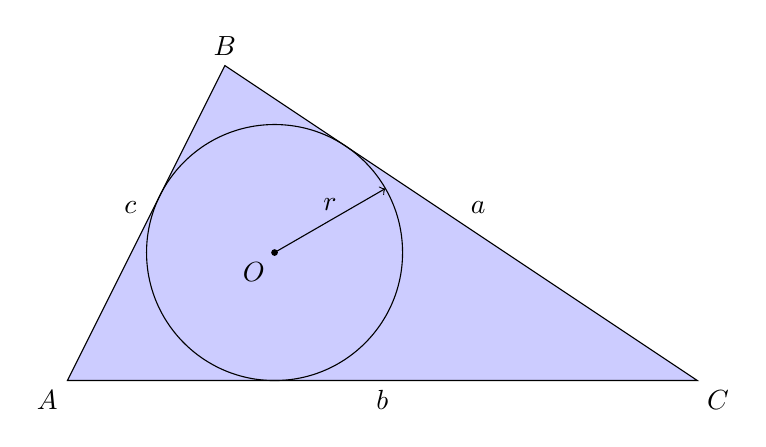
\begin{tikzpicture}

\coordinate (A) at (0,0);
\coordinate (B) at (2,4);
\coordinate (C) at (8,0);

\draw [fill=FilledSurfaceGroupOne] (A) node [below left]{$A$}
      -- node [above left] {$c$} (B) node [above]{$B$}
      -- node [above right] {$a$} (C) node [below right]{$C$}
      -- node [below] {$b$} cycle;

%% Encontrar coordenadas del incentro del triángulo

% Bisectriz interior 1
\coordinate(G1) at ($(A)!1cm!(B)$);
\coordinate(G2) at ($(A)!1cm!(C)$);
\coordinate(M1) at ($(G1)!.5!(G2)$);
% Usamos "10" en ($(A)!10!(M1)$) para asegurarnos que la bisectriz
% interior sea larga y siempre se choque con la otra bisectriz
% interior.
\path[name path=bisc1, overlay] (A) -- ($(A)!10!(M1)$);

% Bisectriz interior 2
\coordinate(H1) at ($(C)!1cm!(A)$);
\coordinate(H2) at ($(C)!1cm!(B)$);
\coordinate(M2) at ($(H1)!.5!(H2)$);
\path[name path=bisc2, overlay] (C) -- ($(C)!10!(M2)$);

\path let \p1=(A), \p2=(B), \p3=(C) in node[overlay] {
    % When you use \p1=(A), TikZ extracts the coordinates in points
    % (pt), where 1 cm≈28.4527
    \xdef\sideAB{\fpeval{sqrt((\x2-\x1)^2 + (\y2-\y1)^2)}}
    \xdef\sideBC{\fpeval{sqrt((\x3-\x2)^2 + (\y3-\y2)^2)}}
    \xdef\sideCA{\fpeval{sqrt((\x3-\x1)^2 + (\y3-\y1)^2)}}
    \xdef\myTriangleSemiperimeter{\fpeval{(\sideAB+\sideBC+\sideCA)/2}}
    \xdef\myTriangleArea{\fpeval{sqrt(\myTriangleSemiperimeter*(\myTriangleSemiperimeter-\sideAB)*(\myTriangleSemiperimeter-\sideBC)*(\myTriangleSemiperimeter-\sideCA))}}
    \xdef\myTriangleInradius{\fpeval{(\myTriangleArea/\myTriangleSemiperimeter)}}
};

\draw [name intersections={of=bisc1 and bisc2, by={centerOfIncircle}}];
% We need to use the unit "pt" explicitly, because the computations
% were done using numbers with units "pt".
\draw (centerOfIncircle) circle (\myTriangleInradius pt);

\draw[fill=black] (centerOfIncircle) circle (1pt) node [below left] {$O$};
\draw[->] (centerOfIncircle) -- node [midway, above] {$r$} ($(centerOfIncircle) + (30:\myTriangleInradius pt)$);

\end{tikzpicture}
\end{document}


